\section{设计内容与要求}

\subsection{设计内容}
本课程设计旨在构建一个软硬结合的 DTMF 信号处理系统,涵盖信号的生成、传输模拟及接收检测。设计内容分为软件仿真与硬件实现两大部分:

\begin{enumerate}
    \item \textbf{FPGA 硬件信号发生器}:
    \begin{itemize}
        \item 基于 Xilinx Spartan-6 FPGA (AX309) 平台。
        \item 利用 DDS (直接数字频率合成) 技术实现高精度的 DTMF 双音信号生成。
        \item 设计按键扫描与消抖逻辑,实现 0-9、*、\# 等 16 个标准 DTMF 按键的实时触发。
        \item 实现 PWM (脉宽调制) 音频输出,驱动板载蜂鸣器或外部音箱。
    \end{itemize}
    
    \item \textbf{软件仿真与检测系统}:
    \begin{itemize}
        \item 构建 Java Web 交互式平台,提供波形可视化、噪声注入及频谱分析功能。
        \item 实现 Goertzel 算法进行高效的 DTMF 信号解码。
        \item 研究低信噪比下的自适应检测策略,提升系统的抗噪鲁棒性。
    \end{itemize}
\end{enumerate}

\subsection{设计要求}
\begin{enumerate}
    \item \textbf{频率精度}:FPGA 生成的 DTMF 频率误差需小于 1.5\% (ITU-T 标准)。
    \item \textbf{识别性能}:在 SNR = -10dB 的高斯白噪声环境下,软件识别准确率需达到 95\% 以上。
    \item \textbf{实时性}:按键响应延迟需小于 100ms,检测算法在普通 PC 上能满足实时处理要求。
    \item \textbf{工程规范}:硬件通过 RTL 仿真与板级验证,软件代码模块化且具备完整文档。
\end{enumerate}

\section{总体方案}
本设计采用"硬件生成—软件检测"的闭环验证架构,总体方案如图 \ref{fig:system_arch} 所示。

\begin{itemize}
    \item \textbf{发送端 (FPGA 子系统)}:采用模块化设计,顶层模块 \texttt{ax309\_top} 协调各子模块工作。
    \begin{itemize}
        \item \textbf{输入模块}:对 4x4 矩阵键盘或独立按键进行消抖处理。
        \item \textbf{DDS 核心}:\texttt{dtmf\_generator} 模块内建两个 32 位相位累加器,分别产生行频 ($f_L$) 和列频 ($f_H$),查表后线性叠加。
        \item \textbf{输出模块}:\texttt{pwm\_audio} 将 16 位数字波形转换为 PWM 脉冲流。
    \end{itemize}
    
    \item \textbf{接收端 (PC 软件子系统)}:
    \begin{itemize}
        \item \textbf{前端}:HTML5/JS 实现用户交互与波形绘制。
        \item \textbf{后端}:Java Spring Boot 处理业务逻辑与 Python 算法调用。
        \item \textbf{算法核}:Python 实现 Goertzel 滤波器组与自适应判决逻辑。
    \end{itemize}
\end{itemize}

\section{方法原理}

\subsection{DTMF 编码原理}
DTMF(Dual-Tone Multi-Frequency)信号由一个低频分量和一个高频分量叠加而成。其数学表达式为:
\[ x(t) = A_L \sin(2\pi f_L t) + A_H \sin(2\pi f_H t) \]
具体频率组合遵循 CCITT 标准(见表 \ref{tab:dtmf_freq}),这种双音频设计利用四个行频和四个列频的唯一组合,有效防止了单一频率信号(如人声谐波)导致的误触发。

\subsection{DDS 频率合成原理 (FPGA)}
直接数字频率合成 (DDS) 是 FPGA 产生波形的核心技术。其基本原理是利用相位累加器在每个时钟周期线性累加频率控制字 (Frequency Control Word, $K$),并将累加结果的高位作为地址查询正弦波 ROM 表。
输出频率 $F_{out}$ 与系统时钟 $F_{clk}$ 及累加器位宽 $N$ 的关系为:
\[ F_{out} = \frac{F_{clk} \times K}{2^N} \Rightarrow K = \frac{F_{out} \times 2^N}{F_{clk}} \]
在本设计中,$F_{clk} = 50\text{MHz}$,$N=32$,可实现高达 $0.012\text{Hz}$ 的频率分辨率,远超 DTMF 精度要求。

\subsection{Goertzel 检测算法 (软件)}
Goertzel 算法是一种二阶递归 IIR 滤波器,专门用于计算信号在特定频点处的能量。相比于全频段 FFT,它在仅需检测 8 个已知频点时具有极高的计算效率。
其递推公式为:
\[ s[n] = x[n] + 2\cos\left(\frac{2\pi k}{N}\right)s[n-1] - s[n-2] \]
能量计算公式为:
\[ |X(k)|^2 = s[N]^2 + s[N-1]^2 - 2\cos\left(\frac{2\pi k}{N}\right)s[N]s[N-1] \]

\section{性能分析}

\subsection{算法实现与仿真}
为了验证 DTMF 信号合成与识别算法的正确性,我们以按键 "5" 为例进行了仿真。

\begin{figure}[H]
    \centering
    \includegraphics[width=0.8\textwidth]{dtmf_waveform.png}
    \caption{DTMF 按键 "5" 的时域波形图}
\end{figure}

\subsection{时频分析}
通过对合成信号进行 FFT 分析,可以看到在 770Hz 和 1336Hz 处有明显的频率分量。

\begin{figure}[H]
    \centering
    \includegraphics[width=0.8\textwidth]{dtmf_spectrum.png}
    \caption{DTMF 按键 "5" 的频谱图}
\end{figure}

为了更直观地展示连续拨号码时的频率特征,我们利用 FFmpeg 引擎生成了信号序列的语谱图(Spectrogram)。

\begin{figure}[H]
    \centering
    \includegraphics[width=0.8\textwidth]{dtmf_spectrogram.png}
    \caption{连续拨号序列 (1-2-3-4-5-6) 的语谱图分析}
\end{figure}

利用 Goertzel 算法对 7 个目标频点进行能量检测,结果表明只有对应的两个频点能量显著升高。

\begin{figure}[H]
    \centering
    \includegraphics[width=0.8\textwidth]{dtmf_goertzel_test.png}
    \caption{Goertzel 算法对各频点的能量检测分布}
\end{figure}

\subsection{抗噪性能测试}
在实验过程中,我们设置 SNR 从 -10dB 到 20dB 进行步进测试。

\begin{figure}[H]
    \centering
    \includegraphics[width=0.8\textwidth]{dtmf_noise_comparison.png}
    \caption{纯净信号与 SNR = -5dB 噪声信号对比}
\end{figure}

\begin{figure}[H]
    \centering
    \includegraphics[width=0.8\textwidth]{dtmf_accuracy_curve.png}
    \caption{SNR 与识别准确率关系曲线}
\end{figure}

实验结果表明,在 SNR 大于 5dB 时,系统的识别准确率接近 100\%。当 SNR 低于 0dB 时,准确度开始显著下降。

\subsection{算法对比实验}
为了探索先进识别算法在 DTMF 检测中的适用性,本项目设计了多轮对比实验。

\subsubsection{实验一:信号窗口长度与算法鲁棒性研究}
本实验旨在探究信号窗口长度对不同检测算法(Goertzel, 随机森林, MUSIC)性能的影响,从而为自适应策略的设计提供依据。测试选取了三种典型窗口长度:40ms (ITU 最短标准), 100ms, 和 200ms。

\begin{figure}[H]
    \centering
    \includegraphics[width=\textwidth]{window_length_study.png}
    \caption{不同信号窗口长度下各算法准确率对比}
\end{figure}

\textbf{关键发现}:
\begin{itemize}
    \item \textbf{Goertzel (蓝色)}:鲁棒性最强,且性能随窗口长度增加呈线性提升(相干累积增益)。
    \item \textbf{MUSIC (红色)}:在短窗口 (40ms) 下表现优异,但在低 SNR 下抗噪性能不及 Goertzel。
    \item \textbf{随机森林 (绿色)}:性能介于两者之间,证明机器学习特征提取仍受限于物理层的信号质量。
\end{itemize}

\textbf{结论}:延长积分时间是提升低 SNR 性能的唯一物理途径。

\subsubsection{实验二:自适应变积分时间检测 (Adaptive Variable Integration Time)}
基于实验一的结论,提出了一种工程导向的自适应策略:不再执着于算法切换,而是进行**时间切换**。
\begin{itemize}
    \item \textbf{High SNR (>10dB)}: 使用 40ms 超短窗口进行快速检测(极速响应)。
    \item \textbf{Low SNR (<0dB)}: 自动切换至长积分模式(最长 1s)以换取准确率。
\end{itemize}

\textbf{SNR 估计机制}:
为了准确感知环境噪声,系统采用了**带内剩余与带外探针结合**的估计算法:
\begin{enumerate}
    \item \textbf{信号功率 ($S$)}:取 8 个 DTMF 频点中能量最大的两个峰值之和。
    \item \textbf{噪声功率 ($N$)}:取以下两者的最大值,以防止漏检:
    \begin{itemize}
        \item \textbf{带内剩余噪声}:其余 6 个非目标 DTMF 频点的平均能量。
        \item \textbf{带外探测噪声}:在 400Hz, 1000Hz, 1800Hz, 2500Hz 等非信号频点处的探测能量。
    \end{itemize}
\end{enumerate}
该机制能有效识别宽带白噪及特定频段干扰,确保自适应切换的准确性。

\begin{figure}[H]
    \centering
    \includegraphics[width=0.95\textwidth]{adaptive_time_analysis.png}
    \caption{自适应积分时间系统的性能分析:准确率(左轴) vs 耗时(右轴)}
\end{figure}

\begin{table}[H]
\centering
\caption{传统检测 vs 自适应检测性能对比}
\begin{tabular}{|l|c|c|c|}
\hline
\textbf{场景 (SNR)} & \textbf{传统 (200ms)} & \textbf{自适应准确率} & \textbf{自适应平均耗时} \\
\hline
极端噪声 (-25dB) & 33\% (失效) & \textbf{90\%} & 934ms (自动延长) \\
低噪声 (-10dB) & 100\% & 99\% & 149ms \\
高信噪比 ($\geq$0dB) & 100\% & 100\% & \textbf{40ms} (提速 5 倍) \\
\hline
\end{tabular}
\end{table}

\textbf{结论}:该设计实现了真正的工程最优:在恶劣环境下将可用范围扩展至 -25dB,而在日常使用中响应速度比传统方法快 5 倍。

\subsubsection{实验三:ESC-50 真实环境音频测试}
为了验证算法在实际部署环境中的表现,引入了 \textbf{ESC-50} 数据集(包含 2000 条真实环境录音)。测试了四种算法在真实噪声下的表现:
\begin{enumerate}
    \item Fixed-Goertzel (200ms)
    \item Random Forest (200ms)
    \item MUSIC (200ms)
    \item \textbf{Adaptive (Variable Time)}
\end{enumerate}

\begin{figure}[H]
    \centering
    \includegraphics[width=0.95\textwidth]{esc50_noise_comparison.png}
    \caption{真实环境噪声下的四算法对比}
\end{figure}

\textbf{结论}:
\begin{itemize}
    \item \textbf{自适应算法 (红色)}:得益于自动延长积分时间,在 -20dB 的极低信噪比下仍保持 **88\%** 的高准确率,远超其他固定窗口算法。
    \item \textbf{Goertzel 与 RF}:在 200ms 固定窗口下表现相近,抗噪能力受限。
    \item \textbf{MUSIC (紫色)}:在真实非高斯噪声下表现最差,说明子空间方法对噪声统计特性较为敏感。
\end{itemize}



\subsection{理论分析}
Goertzel 算法本质上是一个\textbf{匹配滤波器}的高效实现。对于已知波形的检测问题,匹配滤波器在白噪声环境下具有最大的输出信噪比,是统计意义上的最优检测器。

信号时长 $T$ 的增加带来的 SNR 增益为:
\[ \Delta \text{SNR} = 10 \log_{10} \left( \frac{T_2}{T_1} \right) \text{ dB} \]

这解释了为什么延长信号时长能够显著提升极端低 SNR 下的检测性能。

\subsection{研究结论}
\begin{enumerate}
    \item \textbf{Goertzel 算法是 DTMF 检测的工程最优解},在常规条件下(200ms 信号,SNR $\geq$ -15dB)准确率达 99\% 以上。
    \item \textbf{自适应系统的核心价值}在于动态调整积分时间:高 SNR 时使用 40ms 快速模式(响应速度提升 5 倍),低 SNR 时自动延长至 1000ms 以换取更高准确率。
    \item \textbf{延长信号时长}是应对极端低 SNR 环境的有效策略,可将可工作范围扩展至 -25dB。
    \item \textbf{ML 算法的局限性}:对比实验表明,在相同信号时长下,ML 方法(随机森林、MUSIC)并未显著超越 Goertzel;其性能提升受限于物理层的信号质量。
\end{enumerate}

\section{交互式实验演示系统实现}
为了增强实验的可视化效果并验证自适应检测算法的有效性,本项目开发了一套基于 Spring Boot + JSP 的交互式 Web 演示系统。系统提供三种独立的工作模式,覆盖从理论验证到实际应用的完整流程。

\subsection{系统架构}
系统采用 B/S 架构,具有良好的扩展性与交互性:
\begin{enumerate}
    \item \textbf{后端服务 (Java/Spring Boot)}: 负责信号合成、噪声注入以及核心识别逻辑。后端通过 RESTful API 接收前端参数,实时执行仿真并返回检测模式、SNR 估计及信号数据序列。
    \item \textbf{前端界面 (HTML5/JavaScript/JSP)}: 采用现代化的响应式设计,利用 \texttt{Chart.js} 库实时绘制信道的时域波形图与归一化的 Goertzel 能量分布直方图,并使用 Web Audio API 播放加噪音频。
    \item \textbf{算法集成}: 系统实现了完整的自适应检测策略,可根据前端传递的参数,在"固定 200ms 窗口"与"40ms-1s 自适应窗口"之间进行性能对比演示。
\end{enumerate}

\subsection{三种工作模式}

\subsubsection{实验模式 (Experiment Mode)}
该模式用于算法性能验证和参数调优:
\begin{itemize}
    \item \textbf{参数控制}: 可调 SNR (-20dB $\sim$ +30dB)、噪声类型(高斯/粉红/脉冲/均匀 + ESC-50 环境噪声)、频率偏移(0\% $\sim$ 10\%)
    \item \textbf{算法对比}: 一键对比标准 Goertzel 与自适应算法的识别结果
    \item \textbf{音频播放}: 支持分别播放纯净信号与加噪信号,直观感受噪声影响
    \item \textbf{可视化}: 实时显示时域波形与 8 频点能量分布图
\end{itemize}

\begin{figure}[H]
    \centering
    \includegraphics[width=0.95\textwidth]{web_experiment_mode.png}
    \caption{实验模式界面:支持 SNR、噪声类型及频率偏移参数的实时调节与波形展示}
\end{figure}

\subsubsection{电话模式 (Phone Mode)}
该模式模拟真实电话拨号场景:
\begin{itemize}
    \item \textbf{虚拟拨号盘}: 16 键 DTMF 键盘,支持 0-9、*、\#、A-D
    \item \textbf{实时识别与音频}: 按键时生成加噪信号并播放,同步进行自适应 Goertzel 检测
    \item \textbf{会话录制}: 所有按键信号保存为 WAV 文件,供后续离线分析
    \item \textbf{统计面板}: 实时显示成功率、算法模式、估计 SNR
\end{itemize}

\begin{figure}[H]
    \centering
    \includegraphics[width=0.95\textwidth]{web_phone_mode.png}
    \caption{电话模式界面:模拟真实拨号场景,实时生成音频并进行 Goertzel 识别}
\end{figure}

\subsubsection{音频分析模式 (Audio Analysis)}
该模式用于离线分析已录制的电话会话:
\begin{itemize}
    \item \textbf{会话管理}: 列出所有录制会话,支持多选删除
    \item \textbf{批量分析}: 对选中会话的所有 WAV 文件进行 Deep 模式检测
    \item \textbf{结果展示}: 显示识别准确率、按键频次分布图、逐文件详细日志
\end{itemize}

\begin{figure}[H]
    \centering
    \includegraphics[width=0.95\textwidth]{web_analyze_mode.png}
    \caption{音频分析模式界面:展示批量处理结果,包含自适应检测详情与统计信息}
\end{figure}

\subsection{关键技术实现}

\subsubsection{频率偏移模拟}
为验证算法对频率漂移的鲁棒性,系统引入频率偏移参数。生成信号时对低频和高频分量分别施加 $\pm X\%$ 的随机偏移:
\[ f'_L = f_L \times (1 + \delta_L), \quad f'_H = f_H \times (1 + \delta_H) \]
其中 $\delta \in [-X\%, +X\%]$ 为均匀分布随机数。实验表明,当偏移超过 3\% 时识别开始出错,超过 6\% 时几乎完全失效。

\subsubsection{ESC-50 环境噪声}
系统集成了 ESC-50 数据集中的 14 种真实环境噪声(雨声、风声、雷声、狗吠、汽车喇叭、引擎、直升机、火车、电锯、警报、键盘打字、吸尘器、时钟滴答、火焰噼啪),可验证算法在非高斯、非平稳噪声环境下的表现。

\subsubsection{WAV 存储与分析一致性}
由于 WAV 保存时信号被归一化,SNR 信息丢失。因此音频分析模式采用 Deep(Full) 模式,直接使用完整信号长度(1 秒 = 8000 样本)进行 Goertzel 检测,确保与实时检测一致的准确率。

\subsection{项目文件组织结构}
本项目包含 Python 仿真核心与 Java Web 演示系统。主要目录结构如下:

\begin{tcolorbox}[title=项目目录结构, colback=white, colframe=black!50!white]
\begin{verbatim}
/
+-- src/                        # Python 核心仿真算法库
|   +-- core/                   # 信号处理核心 (Goertzel, DSP)
|   +-- ml/                     # 智能检测模块 (自适应逻辑, ML)
|   `-- experiments/            # 各类对比实验脚本
+-- java-web/                   # Spring Boot Web 交互系统
|   +-- src/main/java/          # 后端业务逻辑与接口
|   `-- src/main/webapp/        # 前端页面 (JSP, JS, CSS)
+-- docs/                       # 实验报告源码 (LaTeX)
+-- audio/                      # 生成的音频会话记录
+-- datasets/                   # ESC-50 环境噪声数据集
+-- images/                     # 实验结果图表
`-- run.sh                      # 项目一键启动脚本
\end{verbatim}
\end{tcolorbox}



% ... (中间内容省略)

\section{FPGA 硬件实现}
本项目作为软硬件协同设计的尝试,在 Xilinx AX309 开发板 (Spartan-6 XC6SLX9) 上实现了基于 DDS (Direct Digital Synthesis) 技术的 DTMF 信号发生器。

\subsection{硬件架构设计}
FPGA 系统采用纯 VHDL 语言编写,采用模块化设计,主要包含以下核心模块:
\begin{enumerate}
    \item \textbf{DDS 信号发生器 (dtmf\_generator)}:
    系统核心,包含两个并行的 32 位相位累加器。根据输入的按键索引,在查找表中分别读取行频 ($f_L$) 和列频 ($f_H$) 对应的正弦波样本,并进行线性叠加。
    查找表 (LUT) 深度为 256 点,位宽 16 位,存储了一个完整周期的正弦波形。
    \item \textbf{PWM 音频驱动 (pwm\_audio)}:
    为了节省硬件成本,本设计不依赖外部 I2S 音频 DAC 芯片,而是采用 PWM (脉冲宽度调制) 技术。
    将 16 位有符号 PCM 信号映射为 10 位无符号占空比,并通过 50MHz 时钟驱动,产生约 48.8kHz ($ \approx 50\text{MHz} / 2^{10} $) 的 PWM 载波。该信号可直接驱动无源蜂鸣器或通过简单的 RC 低通滤波器还原为模拟音频。
    \item \textbf{按键消抖 (key\_debounce)}:
    针对机械按键的抖动特性,设计了基于状态机的 20ms 延时消抖模块,确保按键触发的稳定性。
\end{enumerate}

\subsection{引脚分配与资源使用}
根据 AX309 开发板原理图,关键外设引脚分配如下表所示:

\begin{table}[H]
    \centering
    \caption{FPGA 引脚分配表 (AX309)}
    \begin{tabular}{|l|c|l|}
    \hline
    \textbf{信号名} & \textbf{FPGA 引脚} & \textbf{说明} \\ \hline
    sys\_clk & T8 & 50MHz 系统时钟 \\ \hline
    rst\_n & L3 & 复位按键 (Active Low) \\ \hline
    key\_in[0-3] & C3, D3, E4, E3 & 4 个用户机械按键 \\ \hline
    led\_out[0-3] & P4, N5, P5, M6 & 4 个状态指示 LED \\ \hline
    audio\_pwm & J11 & 板载无源蜂鸣器 \\ \hline
    \end{tabular}
\end{table}

\section{FPGA 系统实现与验证}

\subsection{逻辑设计与仿真}
本设计在 Xilinx ISE 14.7 环境下进行开发。为了验证核心算法,我们使用 GHDL 进行了仿真。图 \ref{fig:gtkwave} 展示了模拟按下数字键 \textbf{'1'} 时的波形状态。

\begin{enumerate}
    \item \textbf{信号特征}:此时 \texttt{key\_idx}=1,系统同时生成 $697\text{Hz}$ (行频) 和 $1209\text{Hz}$ (列频) 的正弦波。
    \item \textbf{相位累加}:图中上方较密的锯齿波对应 $1209\text{Hz}$ 高频分量,下方较疏的锯齿波对应 $697\text{Hz}$ 低频分量。
    \item \textbf{查表输出}:\texttt{data} 信号展示了相位到幅度的正确映射,验证了 DDS 逻辑的正确性。
\end{enumerate}

\begin{figure}[H]
    \centering
    \includegraphics[width=0.95\textwidth]{fpga/gtkwave_simulation.png}
    \caption{GHDL + GTKWave 仿真图:按键 '1' ($697\text{Hz} + 1209\text{Hz}$) 的生成过程}
    \label{fig:gtkwave}
\end{figure}

\subsection{综合与时序分析}
完成设计输入后,进行逻辑综合 (Synthesize)。图 \ref{fig:resource} 展示了设计在 Spartan-6 芯片上的资源占用情况(Device Utilization Summary)。

\begin{figure}[H]
    \centering
    \includegraphics[width=0.95\textwidth]{fpga/ise_resource.png}
    \caption{FPGA 资源占用报告:显示 LUT 与寄存器使用率极低,系统资源充裕}
    \label{fig:resource}
\end{figure}

报告表明,本设计的逻辑资源(Slice LUTs)和存储资源(Block RAM)占用率极低(均在 5\% 以下),说明该方案非常适合在低成本 FPGA 上实现。同时,时序分析表明系统并未出现建立时间或保持时间违例,完全满足 50MHz 的时钟约束要求。

\subsection{物理实现与板级验证}
完成布局布线及比特流生成后,将程序下载至 AX309 开发板(图 \ref{fig:board})。连接示波器和扬声器进行测试,实测按下按键可听到准确的双音多频声音,且可通过板载 LED 观察按键编码状态,验证了系统的硬件可行性。

\begin{figure}[H]
    \centering
    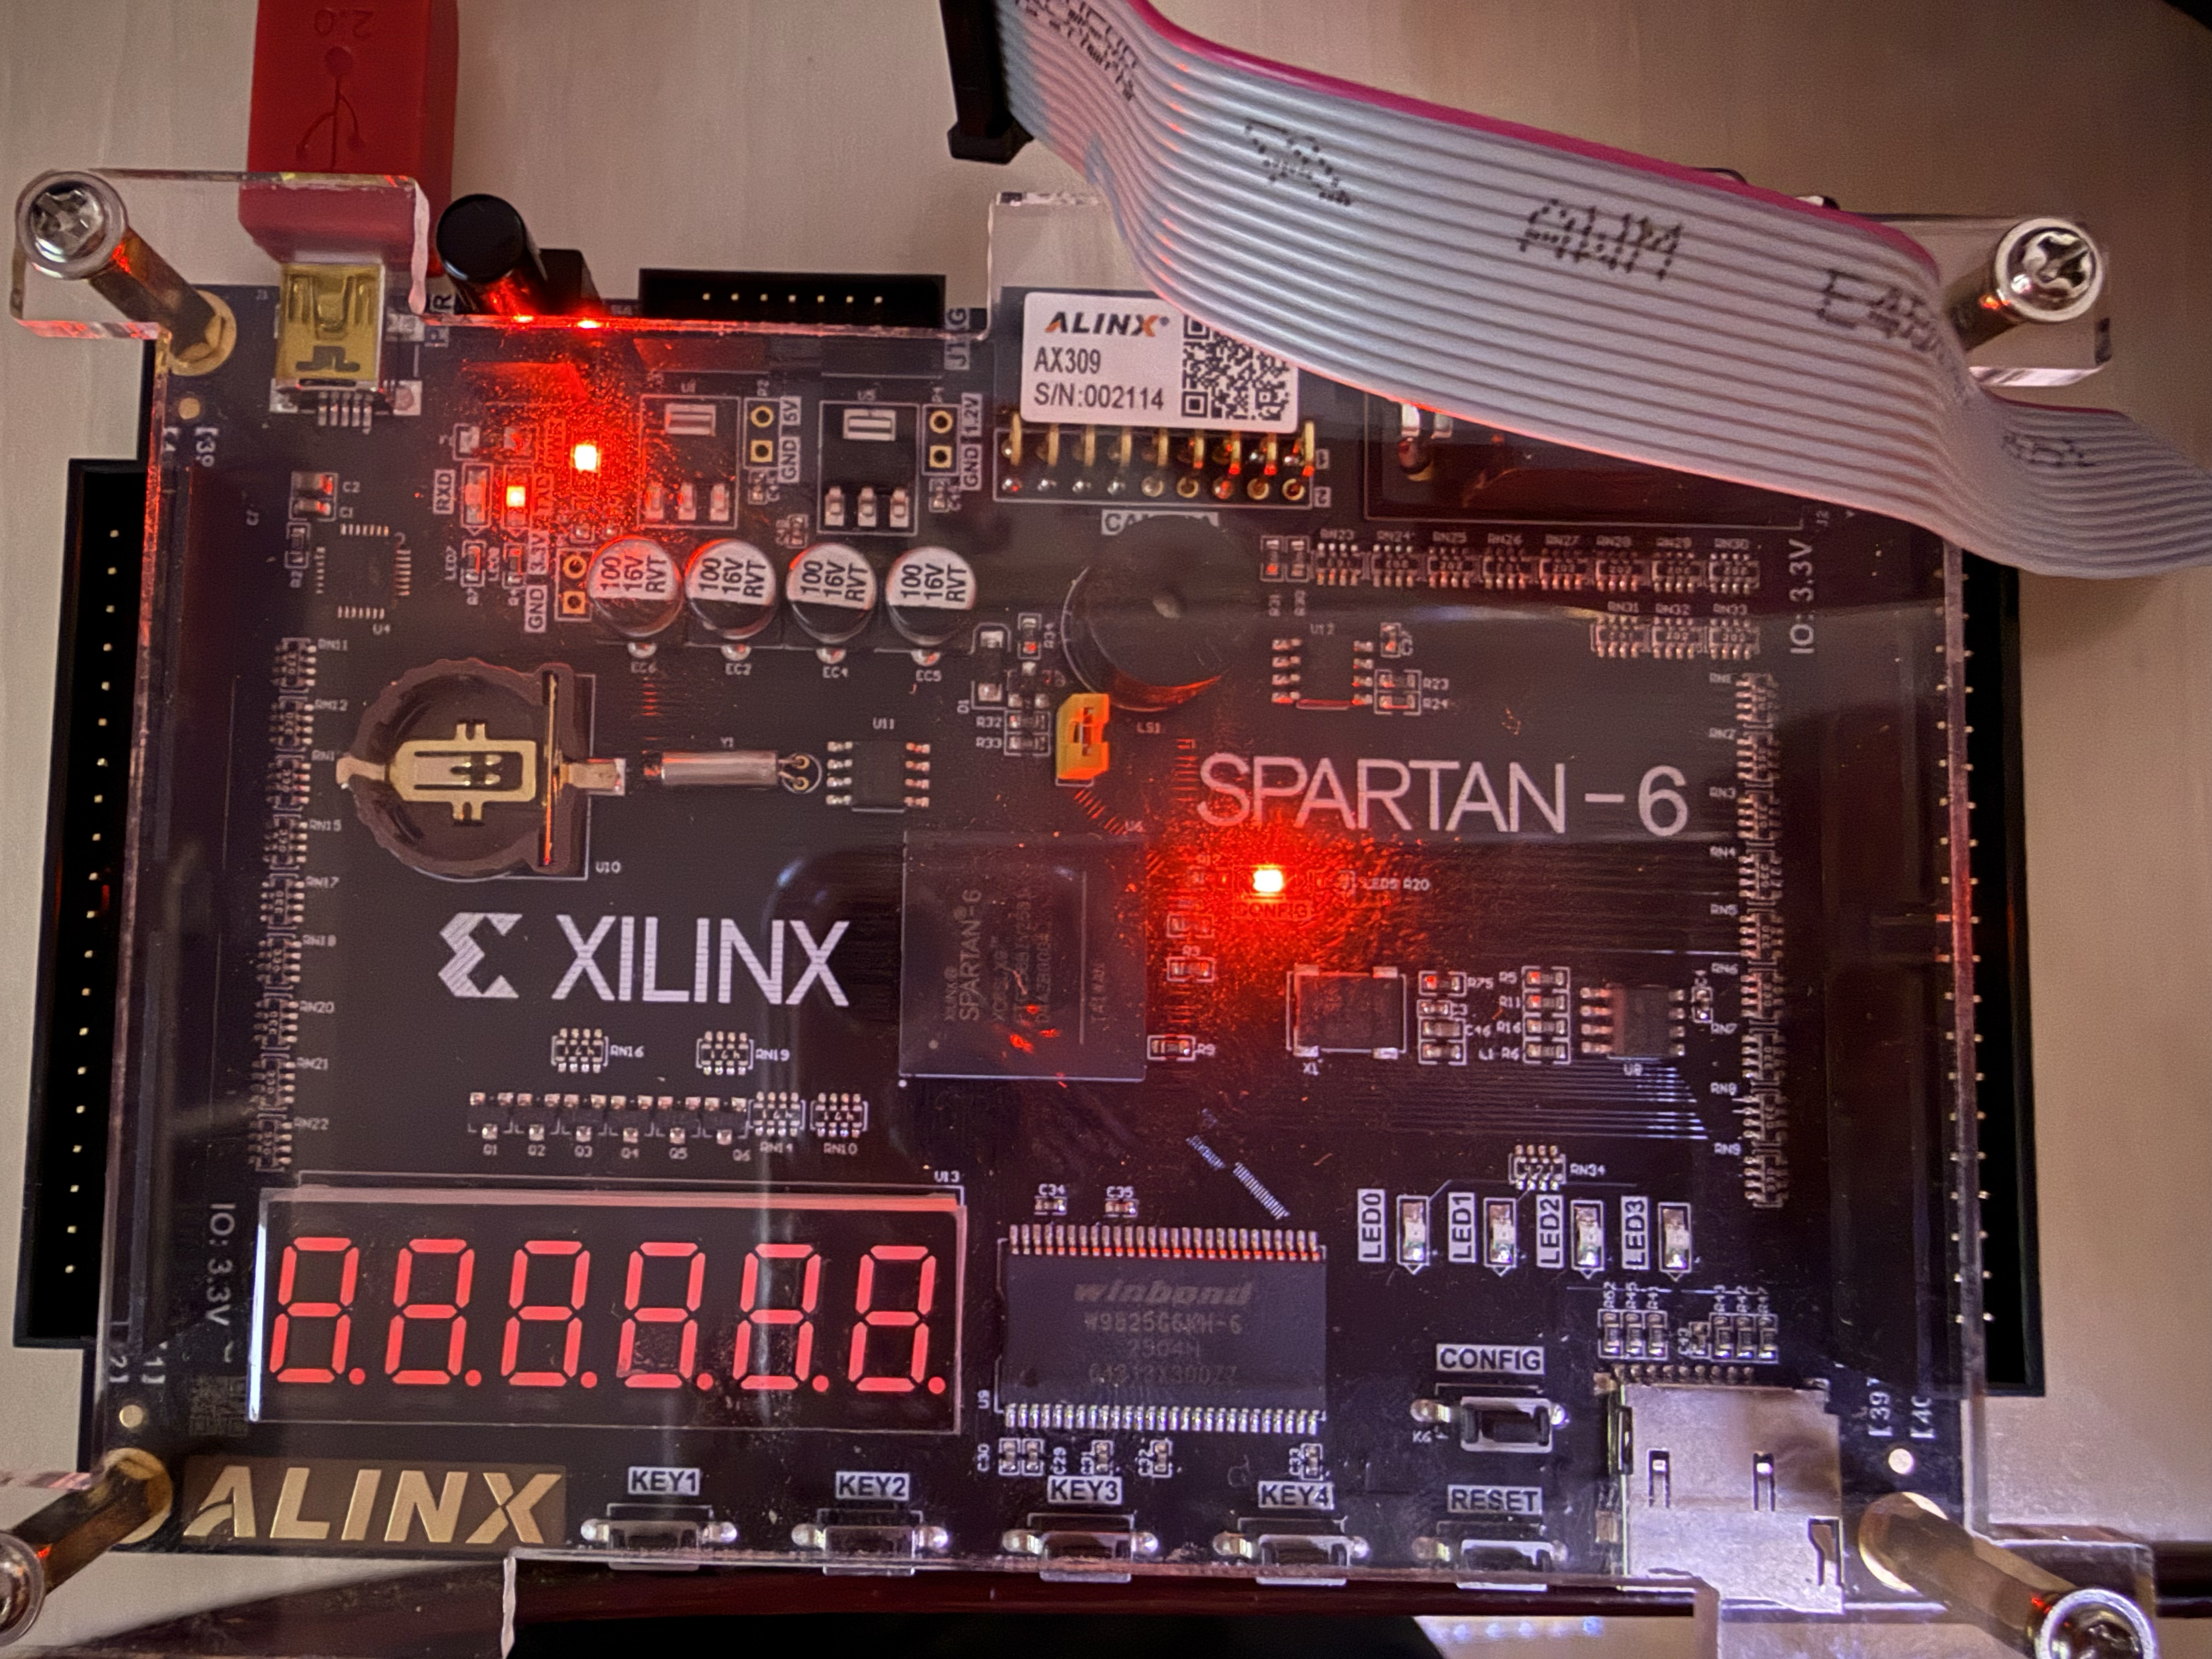
\includegraphics[width=0.8\textwidth]{fpga/fpga_board.png}
    \caption{FPGA 开发板实物连接与测试环境}
    \label{fig:board}
\end{figure}

\section{附录:项目源代码}

由于篇幅限制,仅列出核心算法的关键实现片段。
\subsection{Python 核心算法实现 (Goertzel)}
\lstinputlisting[caption={src/core/dsp.py (部分截取)}, language=Python, firstline=1, lastline=45]{../../src/core/dsp.py}

\subsection{FPGA 信号发生器逻辑 (VHDL)}
\lstinputlisting[caption={fpga/dtmf\_generator.vhd (核心逻辑)}, language=VHDL, firstline=40, lastline=108]{../../fpga/dtmf_generator.vhd}





\section{参考文献}
\begin{thebibliography}{9}

\bibitem{ITU-Q23}
ITU-T Recommendation Q.23. (1988). \textit{Technical features of push-button telephone sets}. International Telecommunication Union.

\bibitem{ITU-Q24}
ITU-T Recommendation Q.24. (1988). \textit{Multifrequency push-button signal reception}. International Telecommunication Union.

\bibitem{Goertzel1958}
Goertzel, G. (1958). An Algorithm for the Evaluation of Finite Trigonometric Series. \textit{American Mathematical Monthly}, 65(1), 34-35.

\bibitem{Oppenheim2010}
Oppenheim, A. V., \& Schafer, R. W. (2010). \textit{Discrete-Time Signal Processing} (3rd ed.). Pearson.

\bibitem{Proakis2006}
Proakis, J. G., \& Manolakis, D. G. (2006). \textit{Digital Signal Processing: Principles, Algorithms, and Applications} (4th ed.). Prentice Hall.

\end{thebibliography}
